
% xetex expected
\documentclass[xetex,professionalfont]{beamer}

% we want math
\usepackage{amsmath}

% fixes and extensions to amsmath
\usepackage{mathtools}

% additional math symbols
\usepackage{amssymb}

% good-looking fractions in text via \sfrac
\usepackage{xfrac}

% fix spaces after custom commands (see below for examples)
\usepackage{xspace}

% minted allows for fancy syntax highlighting (requires python with pygments)
% usage:
%   \begin{minted}{python}
%   codeb
%   \end{minted}
% \usepackage{minted}

% better looking tables
% usage:
%   begin with a \toprule, write a single row of column headings,
%   then add \midrule and after the columns of data we finish with \bottomrule
% example:
%   \begin{tabular}{llr} \toprule
%   Animal & Description & Price \midrule
%   cat & foo & 10 \\
%   dog & bar & 20 \\ \bottomrule
%   \end{tabular}
% note that good tables generally neither have vertical rules nor double rules
\usepackage{booktabs}

% system font support (requires xetex or luatex)
\usepackage{fontspec}
\setmonofont[Scale=0.7]{Cousine} % part of ttf-chromeos fonts on Arch

% improve microtypography
\usepackage{microtype}

% multi-language quotes for babel
\usepackage{csquotes}

% easy way to include copyright information
\usepackage{copyrightbox}

% better bibliographies
\usepackage[backend=biber,style=authoryear]{biblatex}

% language support (english,ngerman)
\usepackage[english]{babel}

% -----------------------------------------------------------------------------

% specify PDF metadata
\hypersetup{pdftitle={CVSP VO - CV History},pdfsubject={},pdfauthor={Christopher Pramerdorfer}}

% copyright font style
\makeatletter\renewcommand{\CRB@setcopyrightfont}{\tiny\color{lightgray}}

% make emph bold
\DeclareTextFontCommand{\emph}{\bfseries}

% use tuwcvl beamer theme
\usetheme{tuwcvl}

% add bib file
\addbibresource{literature.bib}

% -----------------------------------------------------------------------------

% common english abbreviations
\newcommand{\ie}{\mbox{i.e.}\xspace} % i.e.
\newcommand{\eg}{\mbox{e.g.}\xspace} % e.g.

% math - argmin and argmax
\DeclareMathOperator*{\argmin}{arg\,min}
\DeclareMathOperator*{\argmax}{arg\,max}

% shortcuts for number ranges
\newcommand{\NN}{\mathbb{N}}
\newcommand{\ZZ}{\mathbb{Z}}
\newcommand{\QQ}{\mathbb{Q}}
\newcommand{\RR}{\mathbb{R}}

% bold vectors
\renewcommand{\vec}[1]{\ensuremath{\mathbf{#1}}}

% vector shortcuts
\newcommand{\va}{\vec{a}}
\newcommand{\vb}{\vec{b}}
\newcommand{\vc}{\vec{c}}
\newcommand{\ve}{\vec{e}}
\newcommand{\vr}{\vec{r}}
\newcommand{\vs}{\vec{s}}
\newcommand{\vt}{\vec{t}}
\newcommand{\vu}{\vec{u}}
\newcommand{\vv}{\vec{v}}
\newcommand{\vw}{\vec{w}}
\newcommand{\vx}{\vec{x}}
\newcommand{\vy}{\vec{y}}
\newcommand{\vz}{\vec{z}}

% -----------------------------------------------------------------------------

\title{Computer Vision Systems Programming VO}
\subtitle{Computer Vision: Past, Present, Future}
\author{Christopher Pramerdorfer}
\institute{Computer Vision Lab, Vienna University of Technology}

\begin{document}

% -----------------------------------------------------------------------------

\begin{frame}
\maketitle
\end{frame}

% -----------------------------------------------------------------------------

\begin{frame}
\frametitle{Topics}

Selection of past, present, future CV applications\\\medskip
More detailed coverage in upcoming lectures

\bigskip
\begin{center}
	\copyrightbox[b]
	{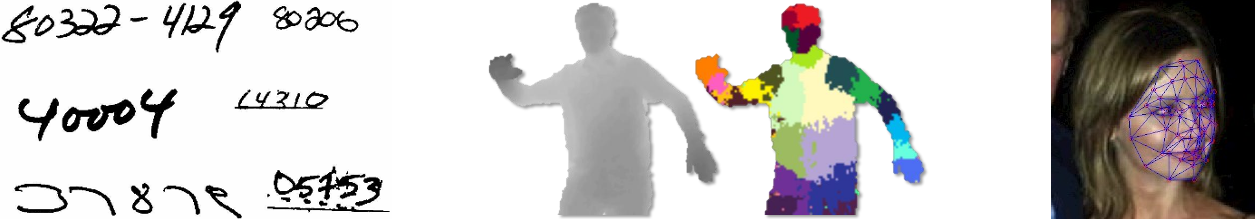
\includegraphics[width=10cm]{figures/intro-collage.png}}
	{\centering Images from \cite{lecun1989}, \cite{shotton2011}, \cite{taigman2013}}
\end{center}

\end{frame}

% -----------------------------------------------------------------------------

\begin{frame}
\frametitle{What is CV?}

Make computers understand images and videos
\begin{itemize}
	\item Different levels of understanding % picture of two persons vs "two professors arguing in front of a blackboard" -> see last slide
\end{itemize}

\bigskip
CV is hard
\begin{itemize}
	\item Inverse (ill-posed) problem % inverse problem = convert measurements into information regarding some world state, ill-posed = (in this context) solution is not unique or sensitive to measurement changes
\end{itemize}

\bigskip
Still, CV has been successfully used in a variety of applications
\begin{itemize}
	\item This lecture introduces a few in chronological order
\end{itemize}

\end{frame}

% -----------------------------------------------------------------------------

\begin{frame}
\frametitle{1963: Pose Estimation}

Edge-based pose estimation of polyhedra \\\medskip % based on relative orientation of edges
Among first CV applications % but not the first as often claimed, see Steve Seitz's slides

\bigskip
\begin{center}
	\copyrightbox[b]
	{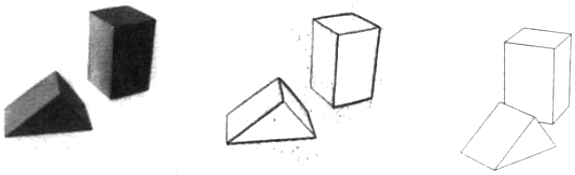
\includegraphics[width=7cm]{figures/blocks-world.png}} % input image, gradient-based edge detection, rendered objects from different viewpoint after recognition
	{\centering Image from \cite{roberts1963}}
\end{center}

\end{frame}

% -----------------------------------------------------------------------------

\begin{frame}
\frametitle{1973: Part-Based Object Detection}

Object representation as parts connected by springs\\\medskip % springs illustrate spatial relations
Known as pictorial structures or constellation models % can be solved in polynomial time via DP if the relation graph is a tree / still used today in improved form

\bigskip
\begin{center}
	\copyrightbox[b]
	{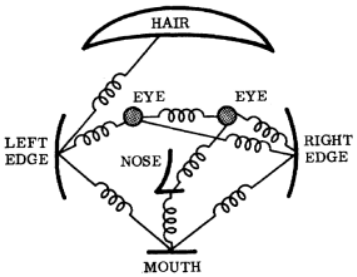
\includegraphics[width=4.5cm]{figures/constellation-model.png}}
	{\centering Image from \cite{fischler1973}}
\end{center}

\end{frame}

% -----------------------------------------------------------------------------

\begin{frame}
\frametitle{1989: OCR via Deep Learning}

% good article on DL history: http://www.wired.com/2014/01/geoffrey-hinton-deep-learning

Zip code recognition from images\\\medskip % from us postal service codes, manual preprocessing to obtain one image per digit
Among first applications using convolutional neural networks % but they had been proposed before, see LeCun's paper

\bigskip
\begin{center}
	\copyrightbox[b]
	{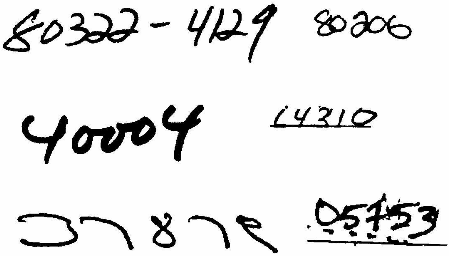
\includegraphics[width=4cm]{figures/zip-numbers.png}}
	{\centering Image from \cite{lecun1989}}
\end{center}

\end{frame}

% -----------------------------------------------------------------------------

\begin{frame}
\frametitle{1989: OCR via Deep Learning}
\framesubtitle{Network Architecture}

\begin{center}
	\copyrightbox[b]
	{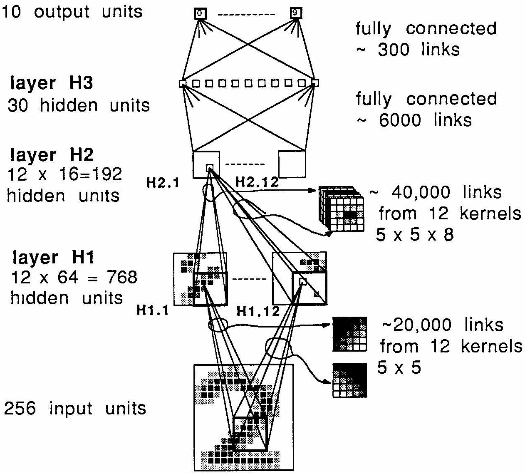
\includegraphics[width=6.5cm]{figures/zip-dnn.png}} % input is 16x16=256, h1 and h2 are convolutional, h3 and output are fully connected. 1256 units, ~65k connections, ~10k params in total
	{\centering Image from \cite{lecun1989}}
\end{center}

\end{frame}

% -----------------------------------------------------------------------------

\begin{frame}
\frametitle{1996: Image-Based Modeling}

Generate a 3D model from a set of images\\\medskip
Use this model and input images to render new images\\\medskip
\url{https://www.youtube.com/watch?v=RPhGEiM_6lM} % Facade introduced view-dependent texture mapping (select "best" images for texturing automatically based on similarity of current and image camera view), used for Matrix bullet-time shots according to video description

\bigskip
\begin{center}
	\copyrightbox[b]
	{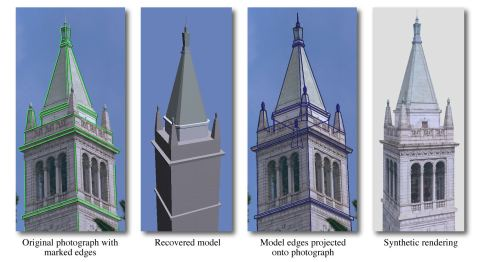
\includegraphics[width=6cm]{figures/facade.jpg}}
	{\centering Images from \cite{debevec1996}}
\end{center}

\end{frame}

% -----------------------------------------------------------------------------

\begin{frame}
\frametitle{2006: Photo Tourism}

3D reconstruction from photo collections\\\medskip
Structure from Motion (SIFT + bundle adjustment) % these things were developed earlier

\bigskip
\begin{center}
	\copyrightbox[b]
	{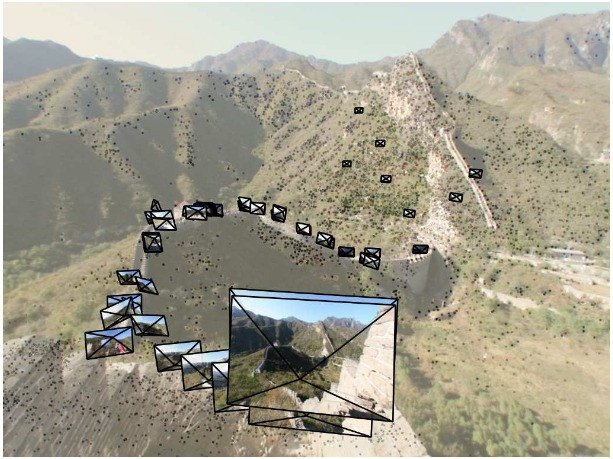
\includegraphics[width=5cm]{figures/photo-tourism.jpg}}
	{\centering Images from \cite{snavely2006}}
\end{center}

\end{frame}

% -----------------------------------------------------------------------------

\begin{frame}
\frametitle{2006: Photo Tourism}
\framesubtitle{Microsoft Photosynth}

\begin{center}
\url{https://photosynth.net}
\end{center}

\end{frame}

% -----------------------------------------------------------------------------

\begin{frame}
\frametitle{2006: Photo Tourism}
\framesubtitle{Building Rome in a Day}

\begin{center}
	\copyrightbox[b]
	{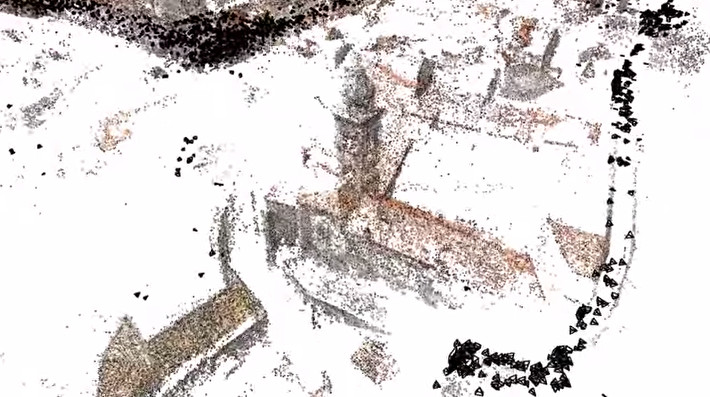
\includegraphics[width=7cm]{figures/dubrovnik.jpg}}
	{\centering Image from \url{https://www.youtube.com/watch?v=sQegEro5Bfo}}
\end{center}

\end{frame}

% -----------------------------------------------------------------------------

\begin{frame}
\frametitle{2007: Smart Digital Cameras}

Cameras with face auto focus\\\medskip
Technology similar to \cite{viola2001}

\bigskip
\begin{center}
	\copyrightbox[b]
	{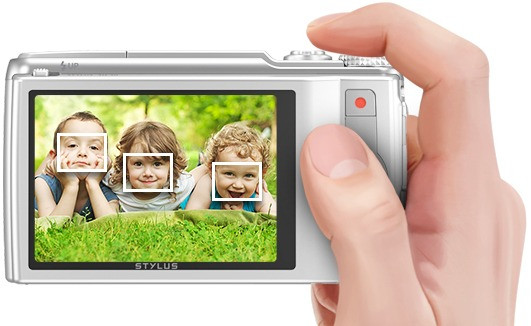
\includegraphics[width=6cm]{figures/camera-faces.jpg}}
	{\centering Image from \url{olympus-europa.com}}
\end{center}

\end{frame}

% -----------------------------------------------------------------------------

\begin{frame}
\frametitle{2011: Kinect}

Depth estimation via active stereo\\\medskip
Real-time pose estimation of multiple players

\bigskip
\begin{center}
	\copyrightbox[b]
	{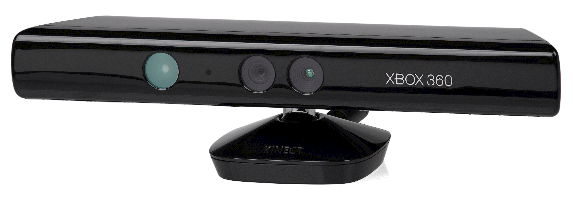
\includegraphics[width=5cm]{figures/kinect.png}}
	{\centering Image from \url{wikipedia.org}}
	\qquad
	\copyrightbox[b]
	{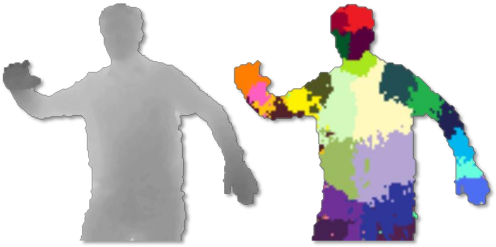
\includegraphics[width=4cm]{figures/kinect-pose.png}}
	{\centering Image from \cite{shotton2011}}
\end{center}

\end{frame}

% -----------------------------------------------------------------------------

\begin{frame}
\frametitle{2013: Human-Level Face Verification}

Face verification using a deep convolutional neural network\\\medskip % face verification is 1:1, i.e. "do image x and y contain the same person or not?"
3D face modeling and frontalization\\\medskip
Verification performance comparable to humans % 120m parameters, compared to LeCun's ~10k

\bigskip
\begin{center}
	\copyrightbox[b]
	{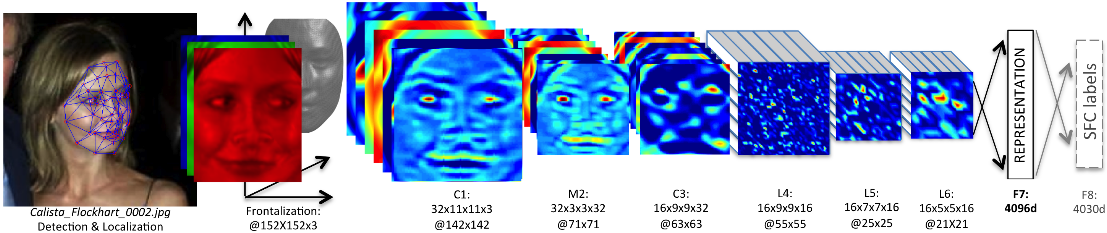
\includegraphics[width=10cm]{figures/deepface.png}}
	{\centering Image from \cite{taigman2013}}
\end{center}

\end{frame}

% -----------------------------------------------------------------------------

\begin{frame}
\frametitle{20xx: Human-Level Object Recognition}

Object recognition without constraints\\\medskip % like occlusions, perspective, background
Hot research topic \scriptsize(\url{http://image-net.org/challenges/LSVRC/2014/index})\normalsize

\bigskip
\begin{center}
	\copyrightbox[b]
	{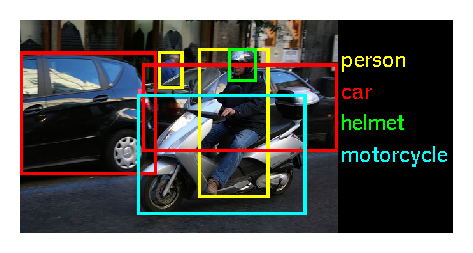
\includegraphics[width=5cm]{figures/object-detection.png}}
	{\centering Image from \url{image-net.org}}
\end{center}

\end{frame}

% -----------------------------------------------------------------------------

\begin{frame}
\frametitle{20xx: Autonomous Cars}

Cars that drive autonomously\\\medskip
Major research area (\eg Google) % with nice progress, but far from everyday application ... there are some good articles on this on the web
\begin{itemize}
	\item \url{https://www.youtube.com/watch?v=bDOnn0-4Nq8}
\end{itemize}

\bigskip
\begin{center}
	\copyrightbox[b]
	{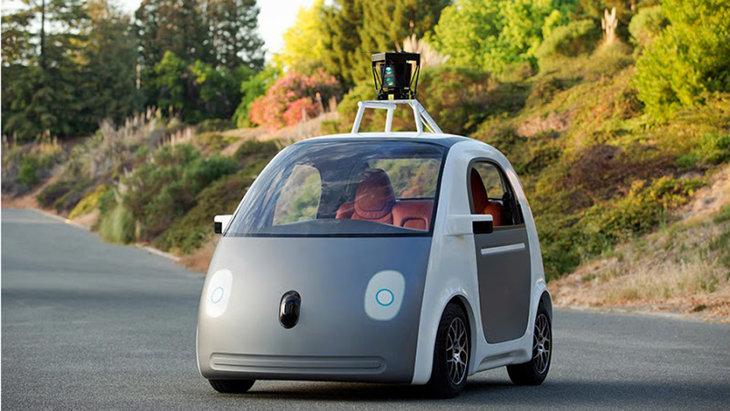
\includegraphics[width=5cm]{figures/google-car.jpg}}
	{\centering Image by Google}
\end{center}

\end{frame}

% -----------------------------------------------------------------------------

\begin{frame}
\frametitle{20xx: Human-Level Scene Understanding}

Object recognition and segmentation, motion, context

\bigskip
\begin{center}
	\copyrightbox[b]
	{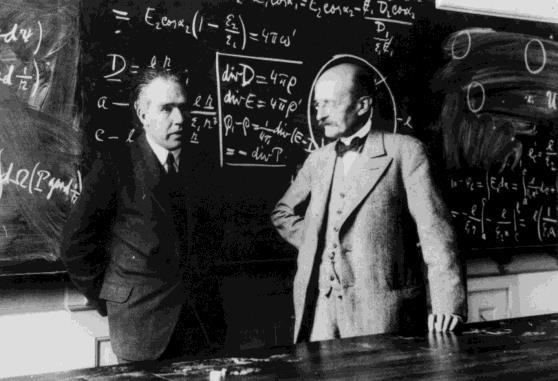
\includegraphics[width=6cm]{figures/planck-bohr.png}}
	{\centering Image from Larry Zitnick's slides}
\end{center}

\end{frame}

% -----------------------------------------------------------------------------

\begin{frame}[allowframebreaks=0.9]
\frametitle{Bibliography}

\printbibliography

\end{frame}

\end{document}
